%% orthologue_conjecture.tex
%% Author: Leighton Pritchard
%% Copyright: James Hutton Institute
%% A brief introduction to orthologues, and their prediction

%
\begin{frame}
  \frametitle{The Ortholog Conjecture
    \footnote{\tiny{Nehrt \textit{et al.} (2011) \textit{PLoS Comp. Biol.} \href{http://dx.doi.org/10.1371/journal.pcbi.1002073}{doi:10.1371/journal.pcbi.1002073
    }}}  
    \footnote{\tiny{Chen \textit{et al.} (2012) \textit{PLoS Comp. Biol.} \href{http://dx.doi.org/10.1371/journal.pcbi.1002784}{doi:10.1371/journal.pcbi.1002784
    }}}  
  }
  \Large{
    \textcolor{olive}{
      \textbf{
      Without duplication, a gene product is unlikely to change its basic function, because this would lead to loss of the original function, and this would be harmful.
      }
    }
  }
\end{frame}

%
\begin{frame}
  \frametitle{The Ortholog Conjecture
    \footnote{\tiny{Nehrt \textit{et al.} (2011) \textit{PLoS Comp. Biol.} \href{http://dx.doi.org/10.1371/journal.pcbi.1002073}{doi:10.1371/journal.pcbi.1002073
    }}}  
  }
  \begin{itemize}
    \item Paralogues are better predictors of function than orthologues \\
      \textcolor{red}{$\therefore$ the conjecture is false}
    \item Cellular context is better for protein function inference
  \end{itemize}
  \textcolor{hutton_green}{(function defined in Gene Ontology (GO) terms)}
    \begin{center}
      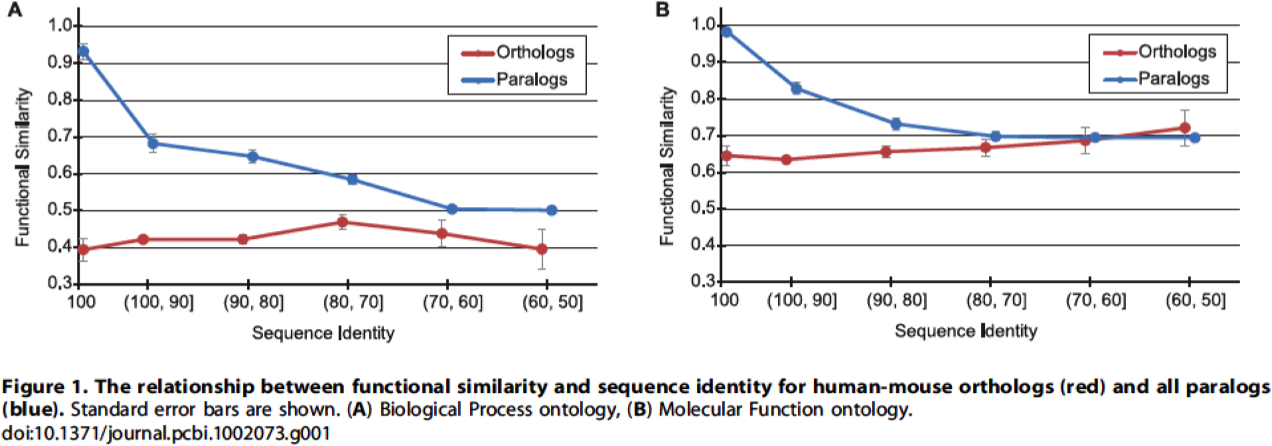
\includegraphics[width=\textwidth]{images/nehrt_orthologues}      
    \end{center}  
\end{frame}

%
\begin{frame}
  \frametitle{The Ortholog Conjecture
    \footnote{\tiny{Chen \textit{et al.} (2012) \textit{PLoS Comp. Biol.} \href{http://dx.doi.org/10.1371/journal.pcbi.1002784}{doi:10.1371/journal.pcbi.1002784
    }}}  
  }
  \textcolor{hutton_green}{We do not understand function well enough to test the conjecture}
  \begin{itemize}
    \item ``examination of functional studies of homologs with identical protein sequences reveals \textcolor{red}{experimental biases, annotation errors, and homology-based functional inferences that are labeled in GO as experimental}. These problems [$\ldots$] make the current GO inappropriate for testing the ortholog conjecture''
    \item Expression level similarity is more similar for orthologues than paralogues \\
    \textcolor{hutton_blue}{(but is this function?)}
  \end{itemize}
\end{frame}